\documentclass[10pt]{article}
\PassOptionsToPackage{hyphens}{url}
\usepackage{hyperref}
\usepackage[margin=0.75in]{geometry}

\usepackage{multicol}
\usepackage{textcomp}
\usepackage{color}
\usepackage{graphicx}
\definecolor{pblue}{rgb}{0.13,0.13,1}
\definecolor{pgreen}{rgb}{0,0.5,0}
\definecolor{pred}{rgb}{0.9,0,0}
\definecolor{pgrey}{rgb}{0.46,0.45,0.48}

\usepackage{listings}
\lstdefinestyle{term}{language=bash,
  columns=fullflexible,
  showspaces=false,
  showtabs=false,
  breaklines=true,
  showstringspaces=false,
  tabsize=2,
  breakatwhitespace=true,
  commentstyle=\color{pgreen},
  keywordstyle=\color{pblue},
  stringstyle=\color{pred},
  basicstyle=\small\ttfamily,
  frame=single,
  moredelim=[il][\textcolor{pgrey}]{$$},
  moredelim=[is][\textcolor{pgrey}]{\%\%}{\%\%},
  upquote=true
}
\lstdefinestyle{sh}{language=bash,
  columns=fullflexible,
  showspaces=false,
  showtabs=false,
  breaklines=true,
  showstringspaces=false,
  tabsize=2,
  breakatwhitespace=true,
  commentstyle=\color{pgreen},
  keywordstyle=\color{pblue},
  stringstyle=\color{pred},
  numbers=left,
  stepnumber=1,
  basicstyle=\small\ttfamily,
  frame=single,
  moredelim=[il][\textcolor{pgrey}]{$$},
  moredelim=[is][\textcolor{pgrey}]{\%\%}{\%\%},
  upquote=true
}

\lstdefinestyle{py}{language=python,
  columns=fullflexible,
  showspaces=false,
  showtabs=false,
  breaklines=true,
  showstringspaces=false,
  tabsize=2,
  breakatwhitespace=true,
  commentstyle=\color{pgreen},
  keywordstyle=\color{pblue},
  stringstyle=\color{pred},
  numbers=left,
  stepnumber=1,
  basicstyle=\small\ttfamily,
  frame=single,
  moredelim=[il][\textcolor{pgrey}]{$$},
  moredelim=[is][\textcolor{pgrey}]{\%\%}{\%\%},
  upquote=true
}

\lstdefinestyle{txt}{
  columns=fullflexible,
  showspaces=false,
  showtabs=false,
  breaklines=true,
  showstringspaces=false,
  tabsize=2,
  breakatwhitespace=true,
  numbers=left,
  stepnumber=1,
  basicstyle=\small\ttfamily,
  frame=single,
  moredelim=[il][\textcolor{pgrey}]{$$},
  moredelim=[is][\textcolor{pgrey}]{\%\%}{\%\%},
  upquote=true
}

\usepackage[T1]{fontenc}

\title{\textbf{Week 04} \\
What is Git
}
\author{
	Melvyn Ian Drag
}
\date{\today}


\begin{document}
\maketitle

\begin{abstract}
We'll learn about git, GitHub, GitLab, and then review grep + regexes.
\end{abstract}

\section{Intro}
You can do tonight's lecture without your digital ocean machine, but starting next week
you will not be able to participate in class without one. Hopefully you got the
homework done and got a machine online. If not, make sure to get it all figured
out by next week because you'll need it.

To get onto your machine from school you need to use a wired connection or use a
hotspot. I would recommend using the school computer - you can ssh from git bash.

\section{git}
\subsection{Essential Concepts}
What you need to know. Don't let me leave here, and don't you leave here,
without me saying the following to you and you having understood it
approximately.

\begin{itemize}
\item why you should learn git
\item what is git
\item how to set up your computer to use git
\item what are unstaged, staged and commited?
\item what are add and commit?
\item what is github?
\item clone, pull, push, fork
\item how to make a pull request on github
\item how to sync your fork with upstream?
\end{itemize}


\subsection{What is git?}
You aren't ready yet young grasshoppers. First we'll get set up, then I'll show
you a few things, then I'll try to explain what is going on.

\subsection{Configuration}
First things first - before we can look at git I want you to set it up. If you
have a digital ocean machine, you must run the following commands:

First install git on linux. I hope youre on digital ocean for tihs class. If
not, git bash has it installed already and I think macs
do too. If they don't then don't worry about it for now, figure it out after
class. Just focus on what we're doing here and take detailed notes to help you
remember. I don't want ot spend 30 minutes waiting for people to install git on
their macs.

Install on digital ocean takes 2 seconds.
\begin{lstlisting}[style=term]
root@yourMachine$ apt update
#stuff happens
root@youtMachine$ apt install git
# it installs
\end{lstlisting}

Now in either git bash ( if you haven't gotten your digital ocean machine up yet
) or on digital ocean, you now need to configure git. You do it like this:

\begin{lstlisting}[style=term]
root@machine$ git config --list
# nothing, you didn't config yet.
root@machine$ git config --global core.editor "vim"
root@machine$ git config --global user.name "James Bond"
root@machine$ git config --global user.email jamesbond@uk.gov
root@machine$ git config --list
user.email=jamesbond@uk.gov
user.name=James Bond
core.editor=vim
\end{lstlisting}

and now you're good to go!

\subsection{Create a repo}
We will now create a git repo. We'll write some code in a directory named
`MyFirstGitRepository'.

Imagine you're working on a big software project. Perhaps your writing a bash
program. Go into your directory and write the following program.

\begin{lstlisting}[style=sh]
#!/bin/bash

echo "Hello world!"
\end{lstlisting}

Now you make this project into a git repository. 

\begin{lstlisting}[style=term]
you@yourComputer$ pwd
/foo/bar/baz/MyFirstGitRepository
you@yourComputer$ ls -a
helloWorld.sh
you@yourComputer$ git init
you@yourComputer$ ls -a
.git helloWorld.sh
you@yourComputer$ # see, now you have a git repository!
you@yourComputer$ git add helloWorld.sh
you@yourComputer$ git commit -m "Finished working on hello world script"
\end{lstlisting}

At this point, your code is backed up with git! What does that mean? Give me a
second I'll show you.

\begin{lstlisting}[style=term]
you@yourComputer$ git log
<Info about your commit!>
you@yourComputer$ git log --oneline
<I like this view of project history better>
\end{lstlisting}

\textbf{Now show class the git log for the lecture notes. They can see all the
work I've been doing on the class notes/homework over the last year or so.}

Now, why is that useful? For a bunch of reasons, I'll show you why that's useful
now. Edit your script such that instead of saying "Hello World" it says `` ciao,
mondo". I guess that's Italian for ``Hello World".

\begin{lstlisting}[style=term]
you@computer$ cat helloWorld.sh
ciao mondo
you@computer$ git add helloWorld.sh
you@computer$ git commit -m "changed language of code"
you@computer$ git log --oneline
<now you see two commits!>
\end{lstlisting}

\textbf{As a class find out how to say `hello world' in other languages? How to
say in Spanish, Tagalog, Arabic, French. Keep changing the file and going
through the add/commit cycle. Each time look at git log --online or git log (
the same info just different presentations, I like the oneline view better)}

Now look at figure ~\ref{fig:checkoutold} to see what we can do with this log
info. We can go back in time. Consider microsoft word - if you write a long
essay for EC101 ( what do they call it here? English Comp 101, right? ) -
imagine you are writing an essay. You might write a long paragraph and then not
like it so you delete it. Then you write a different paragraph. Then you close
the essay and go to sleep. Next day you realize the new paragraph is junk and
want the old one. Too bad, you deleted it. Git allows you to take snapshots of
your code so that you can always go back to checkpoints in youy history. I don't
think you all have ever used a tool as cool and powerful as this.

\begin{figure}[h]
\centering
	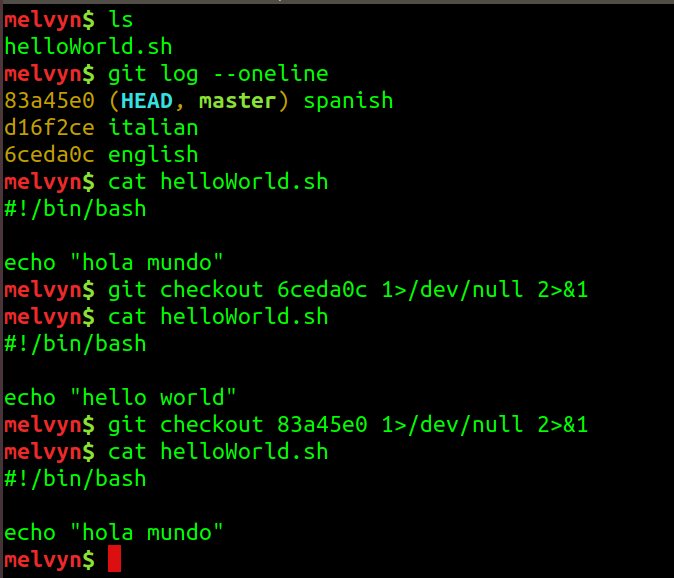
\includegraphics[width=0.8\textwidth]{Images/checkoutOldCommits.png}
	\caption{By using the fingerprint hex number from my commits, I can go back
in time to old commits!! Bet you can't do that with ANY program you know now. }
	\label{fig:checkoutold}
\end{figure}

Explain the difference between:
\begin{itemize}
\item \textit{git add -A}
\item \textit{git add myFile.txt}
\end{itemize}

Now explain, via doodles on the board, the staging area and how commits work. If
you are reading these notes and don't have the benefit of me doodling on the
board to explain this idea, read this:

\url{https://git-scm.com/book/en/v2/Git-Basics-Recording-Changes-to-the-Repository}

and look at the graphics there, this is what I'm following in class, I'mjust
drawing and explaining as I go.


\textbf{So at this point all you know is git. A tiny, but powerful little bit of
git. There is much more to know, but this is the main idea and with just this
you can be very productive. In fact, if you stay in this class you will be very
productive with this bit of knowledge.}

Git is a program you use locally on your computer. That .git directory you can
see with ls -a contains all the hisotry of your code. Pretty cool. But then what
is this github thing? It says `git' in the name, but it also says `hub'. what
the heck?

\section{GitHub}
Github is the server that holds your git repos. You don't need Github to use
git. But imagine this - <anecdote about computer destroyed by milk if time > so
you need to protect yourself against your hardware getting destroyed .You
already do this probably by backing up your images with google photos or iCloud
or whatever the mac equivalent is. Github is like that, but for your git repos.
Laptop dies? You just go to a new computer, clone your code there and then
continue working.


\subsection{First git repo}
Show everyone how to create a git repo. Call it whatever you want and then look
at the instructions it gives you github. You already have a git repo you want to
backup in the cloud - we just made it in the last activity here. Now add a
github remote and push your changes to github as shown on the website. 

\textbf{ Go through the activity with students. Consider making another repo
locally and then pushing it to github.}

Now imagine that your computer is destroyed. Delete your local copy of the repo
to emulate this. rm -r MyFirstGitRepo. 

Now clone the repo and look at git log --oneline. See how all your log history
is preserved? Isn't that great? 

\subsection{How to do Homework}

A common thing to do on github is to make a Pull Request.

There are many many many videos on youtube describing how to do this.

\begin{itemize}
\item This one by a guy who's something of a nerd celebrity \url{https://www.youtube.com/watch?v=rgbCcBNZcdQ}
\item Here's one with a nice accent
\url{https://www.youtube.com/watch?v=dSl_qnWO104}
\item Here's a random one \url{https://www.youtube.com/watch?v=e3bjQX9jIBk}
\item Heres another random one
\url{https://www.youtube.com/watch?v=FQsBmnZvBdc}
\end{itemize}

if you are in class we are going to do some pull requests. \textbf{show the
students the images they can use later for guidance}. Guide the students through
submitting pull requests. Create a folder 

\subsection{Uh oh my fork is out of sync}
When you fork the class repo, you get a snapshot of it at a point in time. You
are adding to this old snapshot and making pull requests that, for very
technical reasons which we are all too tired to think about at the moment,
everything works nicely. I've forcing you to submit your homework in a very
specific way, with a very particular directory structure - this is so that
everything works nice and easy for you and for me.

But as  I was saying, you forked off old code. If you fork today, you have this
weeks code. But between now and next week I'm going to update class materials
for next week. You might not be able ot submit next weeks homework because of
these changes I'm going to make. For this, you need to periodically sync your
fork with my repo.

To do this look in the Images/SyncYourFork directory.

You need to make sure you have an `upstream' remote, then `fetch' it, then it
will merge with yours. Then you are good to go. 

\textbf{Do this with class. Have them all fork, then make a change to the repo,
and have them sync their forks with the repo.}


\section{GitLab, BitBucket, etc.}
There are other things like github. In this class, I think for your final exam,
you will set up a github like website called GitLab. It's relatively
straightforward to install and it looks amazing. The others like BitBucket I
only mention so you've heard of it and won't be confused if you hear some other
programmer talking about it.

\section{grep + regex Review}

\section{8:00 - 8:45 Grep}
Grep is one of the most important command line tools you'll use as a `nix' user,
be it BSD, Linux or MacOS, you need to know Grep. Check out these relevant
videos if you want to know more. One features the man himself, Brian
Kernighan. A major player in the development of Unix and the C language.

\begin{itemize}
\item \url{https://www.youtube.com/watch?v=NTfOnGZUZDk}
\item \url{https://www.youtube.com/watch?v=528Jc3q86F8}
\item \url{https://www.youtube.com/watch?v=6gddK-cOxYc}
\item \url{https://www.youtube.com/watch?v=bKzonnwoR2I}
\end{itemize}

\subsection{8:00 - 8:10 grep revisited}
Now lets look at some more advanced pattern matching used in Linux via the grep command. 
Grep stands for Global regular expression print, it uses regular expressions to search for strings. "What's a regular expressions???" - we'll get to those nasty things in a second, but first we'll take a peek at grep.

Now, grep is immensely useful, as we already saw last week. Last week we typed

\begin{lstlisting}[style=term]
melvyn@thinkpad$ history | grep wget
\end{lstlisting}

to look through our messy bash history to find exactly the command of interest to us, to see what files we downloaded in the past and to potentially download them again.

Probably  100 times a week I use a command that you're now ready to appreciate:

\begin{lstlisting}
melvyn@pc$ history | grep ssh
\end{lstlisting}

I use ssh all week to connect to a handful of differnt machines and can't
remember the ip addressI need to connect to . So I'll just peek in my history
and see what machines I connected to in the past and then reconnect using that
info.

A poem I like:
https://www.cc.gatech.edu/~spencer/poems/woods.txt

You can wget the poem

We are going to cover a bunch of grep options to pick apart this poem.

\begin{enumerate}
\item -i \textit{grep -i HARNESS woods.txt}
\item -w \textit{grep -w arness; grep -wi Harness} 
\item -v for inverse grep i.e. \textit{grep -v arness} 
\item -r mkdir -p a/b; mv woods.txt a/b; grep -r arness *
\item -n grep -rn arness *
\item grep can match lines after + including pattern `grep -A1 arness woods.txt `
\item grep can match lines before and including pattern  `grep -B1 arness woods.txt`
\item grep can match lines around pattern `grep -C3 arness woods.txt`
\item -l to list files containing a pattern \textit{ grep -l arness * }
\end{enumerate}

\begin{verbatim}
remember if we see any irrelevant error messages from grep, we can redirect them to the ether.

     grep -l arness * 2> /dev/null

    e.g.
    
	$mkdir dir
    $grep -l arness *
    grep: dir: Is a directory
    woods.txt
\end{verbatim}   
 
    BUT

\begin{lstlisting}[style=term]    
$grep -l arness * 2>/dev/null
lecture.txt
woods.txt
\end{lstlisting}

A reference for later:
\url{https://opensourceforu.com/2012/06/beginners-guide-gnu-grep-basics/}

\section{8:10 - 8:15 Grep Exercises}
 
Use the above patterns on the file `hamletSolilquy.txt`. See what patterns you can extract. Make sure you test all of the patterns above, as you need to understand grep very well for your homework!

Convince yourself that the flags I've just shown you work:
\begin{itemize}
\item -i
\item -w
\item -v
\item -r
\item -n
\item -A
\item -B
\item -C
\item -l
\end{itemize}

then we'll move on to another interesting part of grep.

\section{8:15 - 8:35 Grep and regular expressions}

Ah, but we have yet to get to regular expressions! Grep stands for
\textbf{Global Regular Expression Print} or \textbf{Generic Regular Expresion
Parser} or something or other, but the "RE" definitely stands for Regular
Expression.

They say when a programmer has a problem and says "I know, I'll use a regular expression!". This is because regular expressions are tricky and easy to screw up if you don't pay attention. The lesson here is the same as with using vim - don't complain that the thing is hard, just learn to use it and then use it without whining! I suspect this proverb is so popular because alot of people don't pay attention to what a regex ( that's short, slang for a regular expression ) is and how to use it. 

Regular expressions are for pattern matching. They are found in every major programming language out there - C++, Python, Java, etc. and you can use them in the bash shell too along with the 'grep' utility.

\url{https://www.gnu.org/software/grep/manual/html_node/Basic-vs-Extended.html}

There are two types - regular and extended. We'll just look at the basic ones - extended is about the same. In your free time click the link above and read it quickly. You'll see they are about the same.

{\Large\textbf{\textit{Note to students:} as with much of what I'll tell you this
semester, I don't have alot of what I'm telling you today memorized. I'm vaguely
aware of the various symbols I'm going to show you and I often have to look at
the documentation before typing anything to amke sure I type it right. It's
important that you understand the concept of a regular expression. Then you'll
be able to use google to figure out exactly what you need to type.}}

In basic regular expressions the meta-characters
\begin{itemize}
\item `?'
\item `+'
\item `\{'
\item `|'
\item `(', and
\item `)'
\end{itemize}

 lose their special meaning; instead use the backslashed versions

\begin{itemize}
\item `\textbackslash?'
\item `\textbackslash+'
\item `\textbackslash\{'
\item `\textbackslash|'
\item `\textbackslash('
\item `\textbackslash)'
\end{itemize}

{\LARGE\textbf{NOTE!! I'll repeat for emphasis - we are using basic regular
expressions in this lesson. So if we want to use the `+' meta-character we have
to instead type `\textbackslash+'}}

What to know:
\begin{enumerate}
\item The period (.) matches any single character.
\item ? means that the preceding item is optional, and if found, will be matched at the most, once.
\item * means that the preceding item will be matched zero or more times.
\item + means the preceding item will be matched one or more times.
\item {n} means the preceding item is matched exactly n times, while {n,} means the item is matched n or more times. {n,m} means that the preceding item is matched at least n times, but not more than m times. {,m} means that the preceding item is matched, at the most, m times.
\end{enumerate}

Some more syntax:
\begin{enumerate}
\item \textasciicircum (Caret)   =   match expression at the start of a line, as
in \textasciicircum\,A will match an A at the beginning of a line.
\item $ (Dollar sign)    =   match expression at the end of a line, as in A$.
\item \textbackslash (Back Slash)  =   turn off te special meaning of the next character, as in \^.
\item [ ] (Brackets)  =   match any one of the enclosed characters, as in [aeiou]. Use Hyphen "-" for a range, as in [0-9].
\item . (Period)  =   match a single character of any value, except end of line.
\item * (Asterisk)    =   match zero or more of the preceding character or expression.
\item \{x,y\} =   match x to y occurrences of the preceding.
\item \{x\}   =   match exactly x occurrences of the preceding.
\item  \{x,\}  =   match x or more occurrences of the preceding.
\item \begin{verbatim}[\^ ]    =   match any one character except those enclosed in [ ], as in
[\^ 0-9].\end{verbatim}
\end{enumerate}

That's it! So, given the file a.txt ( see this directory )

We can do the following

\begin{lstlisting}[style=term]
$ grep "a" a.txt # Find lines with an a
$ grep "a\?" a.txt # find lines with an optional a.
$ grep "a?" a.txt # find lines containing a?
$ grep "a\+" a.txt # find lines with 1 or more "a"s
$ grep "a+" a.txt # find lines  containing "a+" 
$ grep "a$" a.txt # find lines that end with a
$ grep "[0-9]$" a.txt # find lines that end with a number
$ grep "^[a-zA-Z]$" a.txt # find lines with one letter.
$ grep "a\{2,\}" a.txt # find lines with 2 or more "a"s
\end{lstlisting}



\end{document}
